\documentclass[technical_document.tex]{subfiles}
\begin{document}
\section{Software design}
Before writing the code for Eva, a software node design was made to gain insight about the structure of the software to be 
implemented. This structure was modeled to the master-slave model \footnote{http://en.wikipedia.org/wiki/Master/slave\_(technology)} . Each package in this structure represent a physical 
part of Eva, with a logical\_unit package acting as her ``brain'' which receives data from Eva's sensors and make decisions 
based on the readings. The package input is used to read out sensor data such as the Microsoft Kinect and microphone. The 
decisions made by the logical\_unit result in actions that have to be executed by the physical parts of Eva, in other 
words, the logical unit will generate commands for the other packages to execute. Figure \ref{fig:concept} shows the initial design of the software packages.

Looking inside each package, each package has a ``Controller'' node which is essentially the master of the package. An exception is the input package, which is used to read out and stream sensor data for processing. Each ``Controller'' node listens to data from its own master and uses that data to control its own subordinates, resulting in low-level motor control or control of other devices such as the LEDS in Eva's head etc. In this structure, the main Controller of the whole software structure is the Controller in the logical\_unit, since that is, as mentioned before, Eva's brain, whereas the ``AutonomeControllers'' are only masters within their own package. This means that this structure is not simply a master-slave model, but a master-submaster-slave model, with one master in the logical unit, submasters in each package and the rest of the nodes acting as slaves (with the exception of the ndoes in the input package). 

The logical\_unit is special in the sense that it consists of two subpackages, the sense\_component and the action\_component. The idea was that the sense\_component would process all incoming sensor data, while the action\_component would be an extendable database of certain actions that can be executed by the Controller. However, this has changed in the implementation as will be discussed in the next section \ref{sec:implementation}. 

In software engineering, designs should be loosely coupled, yet highly cohesive \footnote{http://www.xyzws.com/scjp/SGS11/5/2} . In this design, loose coupling was automatically achieved because of the ROS framework. In ROS, nodes communicate with each other through topics or services. A node can call a service on another node, or it can post its data on a topic which is accesible for any node in ROS. Especially when topics are used, these nodes can run completely independent from the other nodes, making the entire system loosely coupled. One could remove a node in the ROS system without destroying other nodes and replace it with another one. As long as this new node keeps the protocol between the old node and the rest of the system intact (meaning that it listens and broadcasts to the same topics or services), this node may have an entirely different implementation.

High cohesion is achieved by splitting the software in packages with a specific task. As mentioned before, each package represents a physical ``body'' part of Eva, such as her arm, mobile base, sensors etc. This way, each package is specialized in one part of the robot and only contains nodes to provide functionality within that package and one node to communicate with the rest of the system (the Controller node in that package).

\begin{figure}[h!]
	\centering
	\mbox{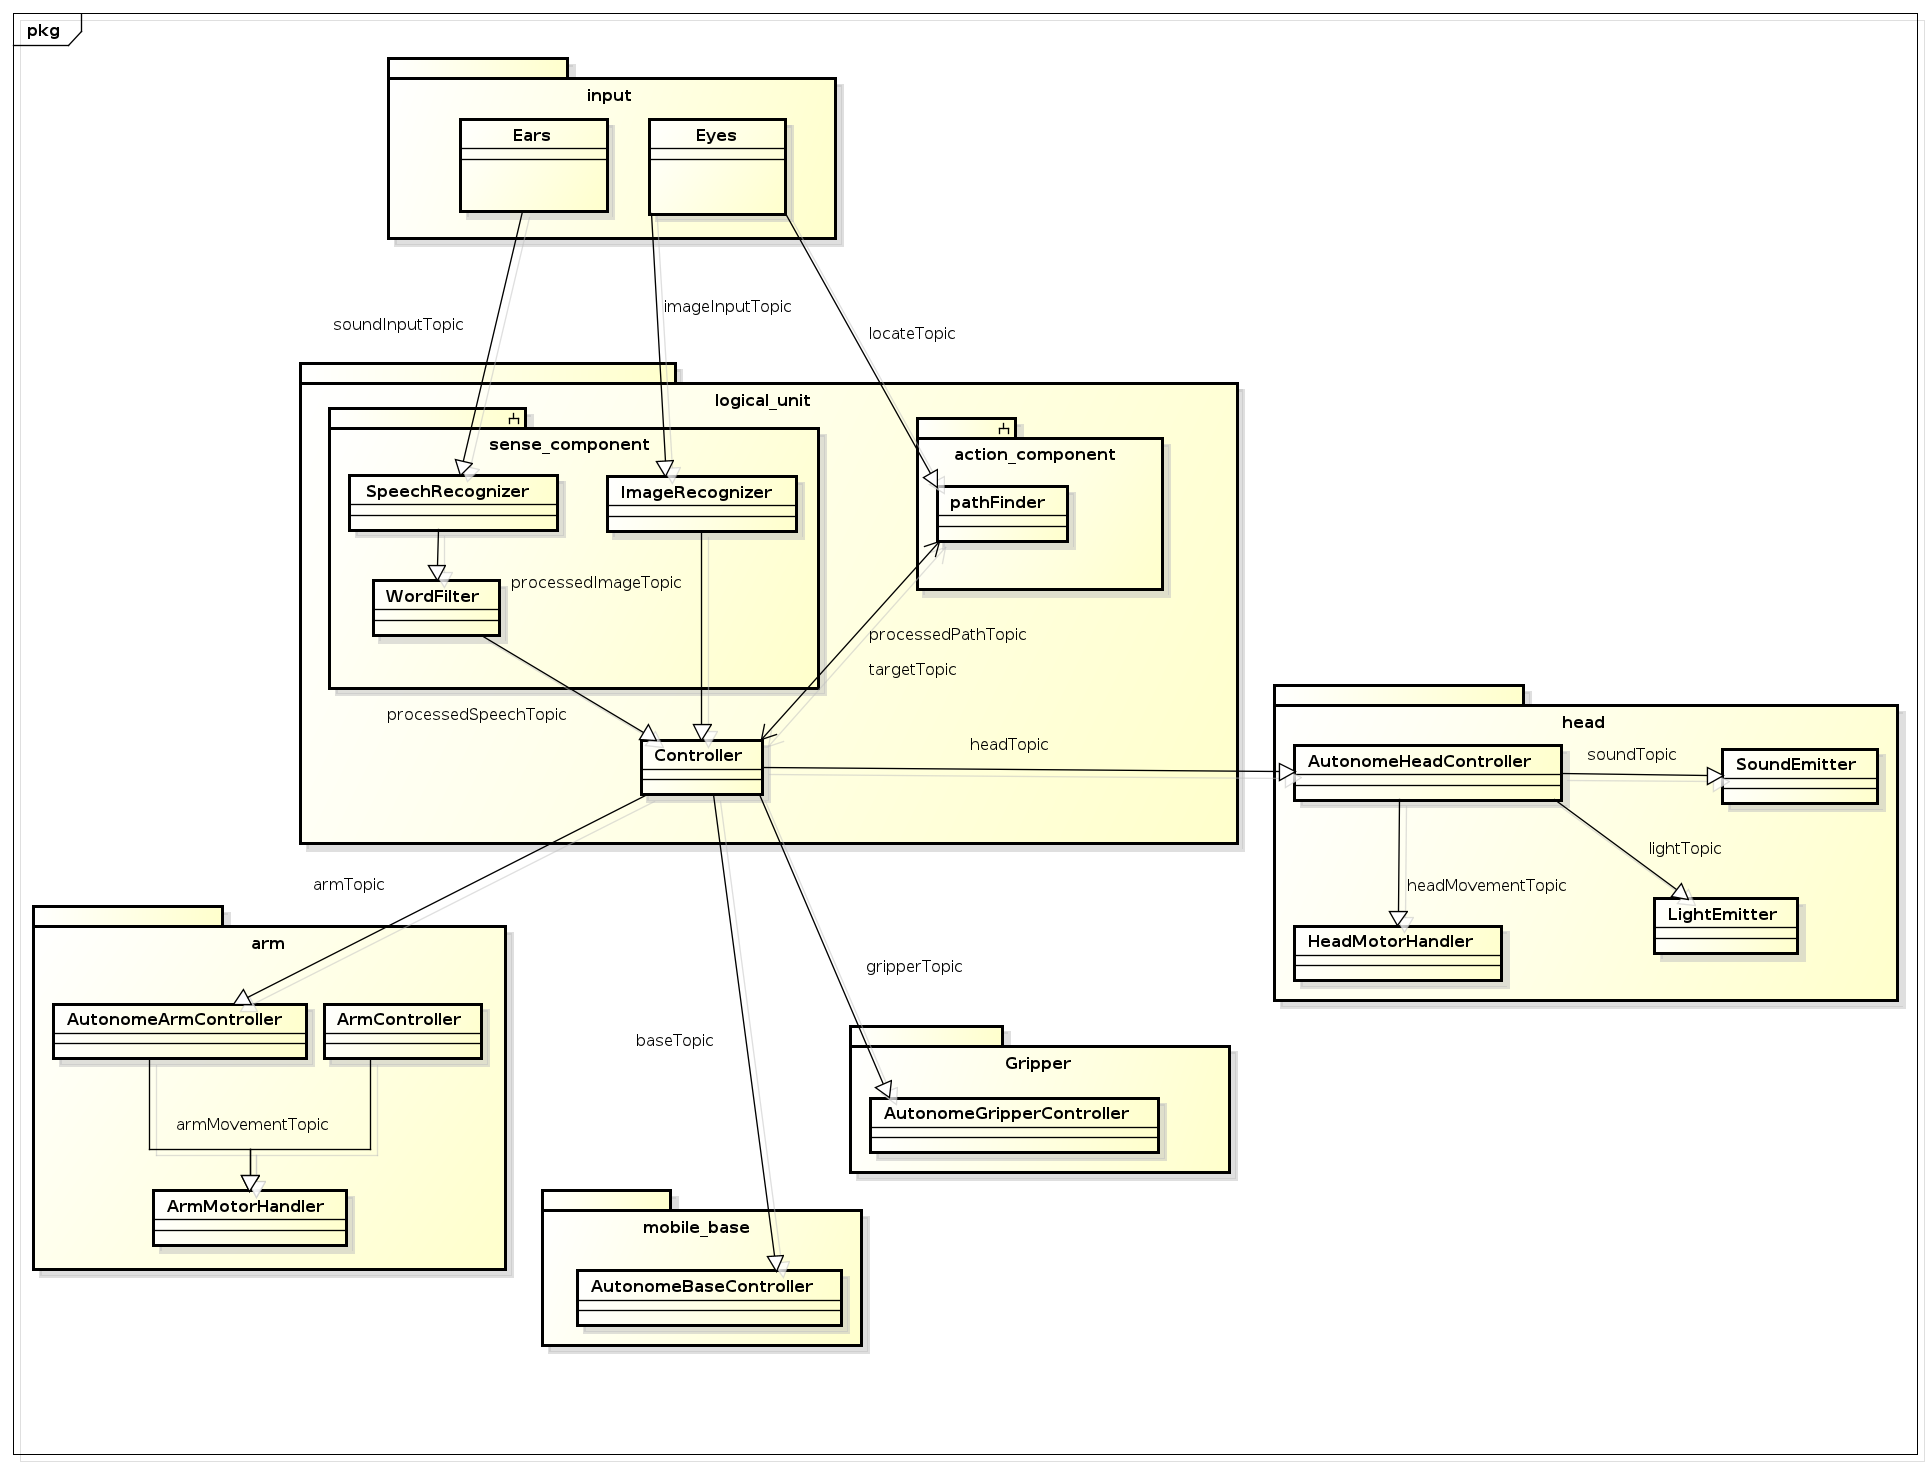
\includegraphics[scale=0.3]{Images/Node_structure.png}}
	\caption{Structure of the packages of the initial design and the nodes within it.}
	\label{fig:concept}
\end{figure}

\section{Software implementation}
\label{sec:implementation}
Using the design discussed in the previous section, Eva's software was built. However, just like with every software project, the final implementation differs from the initial design. The master-submaster-slave structure can still be seen in the implementation, but it is improved by having the slaves provide direct feedback to the master of the system. This way, the master in the logical\_unit can adjust to the data provided by the slaves, resulting in better control of the whole system. Also, the input package is split apart in two different packages: image\_processing and audio\_processing, increasing the cohesion of the entire system. It is a good sign that only few changes have been made to the original design, which means that the initial idea was designed well. The node structure of the implementation can be seen in figure \ref{fig:implementation} ; External packages implemented by third parties are shown in the notes in the figure.

\begin{figure}[ht!]
	\centering
	\mbox{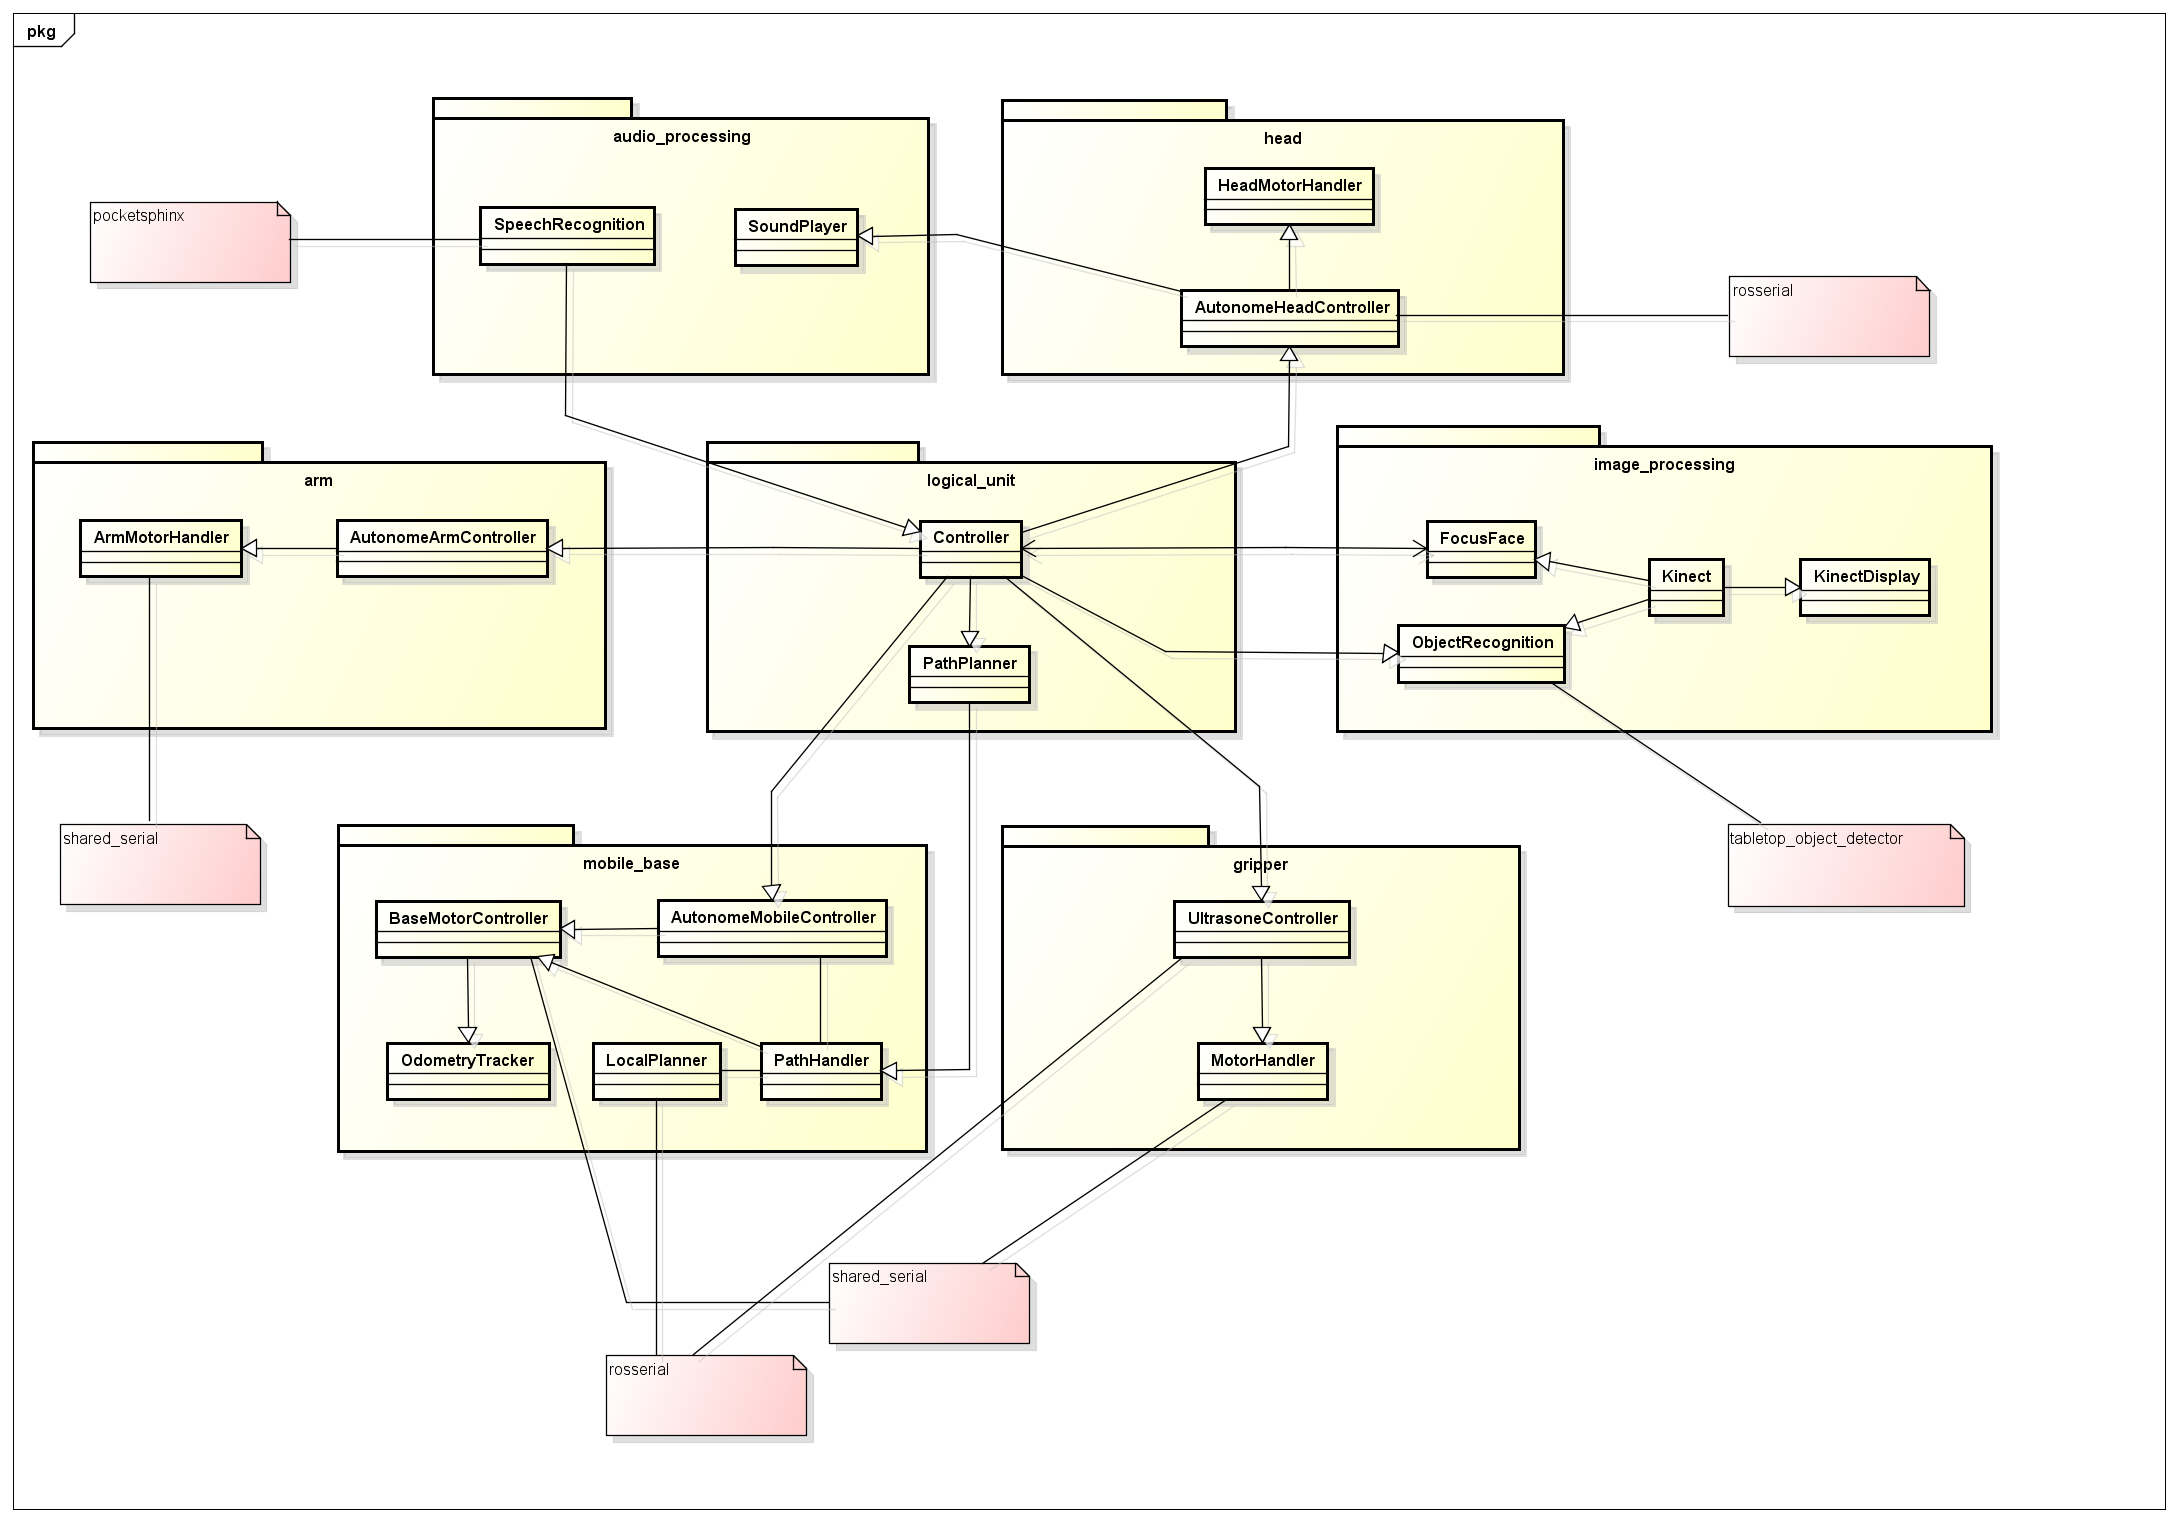
\includegraphics[scale=0.3]{Images/nodes.png}}
	\caption{Structure of the packages as in the implementation and the nodes within it.}
	\label{fig:implementation}
\end{figure}

\end{document}

